%% Dokumentklasse KOMA-Script Report
\documentclass[paper=a4, 12pt, twoside]{scrreprt}
% report zweiseitig gemacht!
%% Encoding UTF8
\usepackage[utf8]{inputenc}
%% 8 Bit Aufloesung der Buchstaben
\usepackage[T1]{fontenc}
%% Seitenraender
\usepackage[scale=0.72]{geometry}
%% Spracheinstellungen
\usepackage[english, naustrian]{babel} % your native language must be the last one!!
%% erweiterte Farbenpalette
\usepackage[dvipsnames]{xcolor}
%% Abbildungen
\usepackage{graphicx}
%% Tabellen (erweitert)
\usepackage{tabularx}
%% TikZ + Circuit-TikZ (fuer Schaltungen)
\usepackage[europeanresistors, europeaninductors]{circuitikz}
%% Nuetzliche TikZ Libraries
\usetikzlibrary{arrows, automata, positioning}
%% mathematik
\usepackage{amsmath, amssymb}
%\usepackage{mathtools}	
%% pdf-einbindung
\usepackage{pdfpages}
%% scource-code einbindung
\usepackage{listings, scrhack} %scrhack vermeidet Umschaltung auf KOMA Floats..
\usepackage{courier}
%% euro-symbol
\usepackage{eurosym}
%% landcsape-seiten ermöglichen
\usepackage{lscape}

%% Diplomarbeits-Format
\usepackage{srdpdipa}

%% Abkuerzungsverzeichnis
\usepackage[]{acronym}

%% Todos
\usepackage[]{todonotes}

%% Ganttdiagramme
\usepackage{pgfgantt}

%% Subfigures
\usepackage[lofdepth]{subfig}

%% Quotes
\usepackage{csquotes}

%%Comments
\usepackage{comment}
\excludecomment{comment}

%% Für figures (H)
\usepackage{float}

%% Bei Bildern für valign
\usepackage[export]{adjustbox}

\usepackage[justification=centering]{caption}

%% definitionen =====================================%%
\dataSchool{HTBLuVA St. Pölten}
\dataDepartment{Höhere Lehranstalt für Elektronik und Technische Informatik}
\dataSubdepartment{Ausbildungsschwerpunkte Embedded- \& Wireless Systems}
\dataSession{2016/17}

\title{Bluetooth-Aktivbox}
\author{Markus Bointner \and Andreas Macsek}
\date{\today}
\place{St. P\"olten}
\professor{Prof. Dipl.-Ing. Dr. Herbert Wagner}
%%====================================================%%

% Hyperlinks im Dokument
\usepackage[colorlinks=true,
    linkcolor=black,
    citecolor=green,
    bookmarks=true,
    urlcolor=black,
    bookmarksopen=true]{hyperref}

\begin{document}

\frontmatter

%% titelseite ==========================================%%
\maketitle
%%======================================================%%

%% komplett leere seite ================================%%
\newpage\null\thispagestyle{empty}%\newpage
%%======================================================%%

%% eidesstattliche erklärung ===========================%%
\begin{affidavit}
    \unterschrift{Markus Bointner}
    \unterschrift{Andreas Macsek}
\end{affidavit}
%%======================================================%%

%% dokumentation (deutsch/englisch) ====================%%
\includepdf[pages=-]{form/dokumentation-de.pdf}
\includepdf[pages=-]{form/dokumentation-en.pdf}
%%======================================================%%

%% inhaltsverzeichnis ==================================%%
\tableofcontents
%%======================================================%%

%% HAUPTTEIL ===========================================%%
\responsible{Markus Bointner, Andreas Macsek}
\mainmatter

% Allgemeines über die Diplomarbeit
\chapter{Einleitung}
In diesem Kapitel wird erläutert, wie die Idee für diese Diplomarbeit entstanden ist und warum sie auch so verwirklicht wurde.

\section{Erste Idee} \label{sec:1.1}
Das Grundkonzept stammt von uns, also Markus Bointner und Andreas Macsek. Da wir beide von Musik begeistert sind, dachten wir uns, dass es sehr interessant wäre selbst eine Lautsprecherbox zu entwickeln. Gleich zu Beginn war klar, dass wir noch ein kleines Extra mit einbauen wollten: eine Bluetooth-Ansteuerung.

\section{Weiterführende Gedanken} \label{sec:1.2}
Um all unsere Ideen zu verwirklichen haben wir entschieden, diese Diplomarbeit ohne Firma und für den privaten Gebrauch zu entwickeln. Genauer gesagt ist die Box dafür gedacht, im Freien oder in größeren Räumen, die Musik für kleinere Menschenmengen bereitzustellen. Das soll auch ohne externe Stromzufuhr möglichst einfach funktionieren. Aus diesem Grund entstand dann die Idee einen Akku zu verbauen. Die einfache Bedienung soll mithilfe eines Bluetooth-Moduls verwirklicht werden.


% Ziel der Diplomarbeit
\chapter{Gesamtprojekt}
\section{Ziele}\label{sec:2.1}
Es soll ein 2.1-System entwickelt werden.
Ein Mono-Subwoofer übernimmt den niedrigen Audiofrequenzbereich, während 2 weitere Lautsprecherboxen (auch genannt Satelliten-Boxen) - mit jeweils einem Hochton- und Tiefton-Lautsprecher - den Rest übernehmen.
Dieser Aufbau wurde gewählt um einen Raum-Klang erzeugen zu können. \\
Die Versorgung der Elektronik erfolgt entweder über Akku- oder Netzbetrieb.
Jeder Hochton- und Tiefton-Lautsprecher bekommt einen eigenen Verstärker (so auch der Mono-Subwoofer). \\
Das Audiosignal wird in verschiedene Frequenzbereiche aufgeteilt.\\

%An Struktur neu anpassen
Unsere Diplomarbeit kann grob in 2 Teile aufgeteilt werden:
\begin{itemize}
	\item Entwicklung der Elektronik
	\item Auswahl und Messungen der Lautsprecher
\end{itemize}
Die Ziele der 2 Teile werden in diesem Kapitel kurz erläutert.

\subsection{Elektronik}\label{subsec:2.1.1}
Wie bereits in der Einleitung (\ref{sec:1.2}) erwähnt, ist das Projekt auch für Akkubetrieb ausgelegt und benötigt daher eine passende Versorgungsschaltung.
Das Versorgungskonzept sieht einen 12V-Akku mit entsprechendem Ladegerät vor.
Dieses wurde zugekauft, da unser Projekt sich auf die Lautsprecher konzentriert.
Bei Anschluss an eine Steckdose (nach EU-Norm) übernimmt das vorgesehene Netzteil die Versorgung der Elektronik.
Wegen einer höheren Versorgungsspannung als 12V, steht bei Netzbetrieb eine höhere Leistung zur Verfügung. \\ \\
Es werden analoge Verstärker verwendet.
Gründe dafür sind:
\begin{itemize}
	\item Einfacher Aufbau
	\item Genügend Leistung und Effizienz für dieses Projekt
	\item Bewährte Technik für Audioverstärker
\end{itemize} 
Das Audio-Signal muss vor den Verstärkern natürlich noch gefiltert werden. Diese Aufgabe übernimmt eine Aktive Frequenzweiche. Für den Mono-Subwoofer wird eine eigene Schaltung entwickelt die nicht nur die unerwünschten Signal-Anteile herausfiltert, sondern auch noch das Stereo-Signal auf ein Mono-Signal addiert. \newpage
Die Signalaufnahme erfolgt über ein Hauptboard mit dem Bluetooth-Modul, welches während einer Projektarbeit in der HTBLuVA St. Pölten entwickelt wurde. Darauf befindet sich außerdem noch ein Klinkenanschluss und eine Addierschaltung.

\subsection{Lautsprecher}\label{subsec:2.1.2}
Das Ziel für die Auswahl der Lautsprecher war es, möglichst laute Chassis mit möglichst gutem Frequenzgang (wenig Schwankung, möglichst waagrecht) zu finden. Ein weiteres Ziel ist die Verringerung des Volumens der Box, wobei dennoch eine gute Klangqualität erhalten bleibt. Ein kleines Volumen ist nötig, da das fertige System auch für den Außenbereich verwendet werden soll und daher tragbar sein sollte.        
    
% Erklärung verwendeter Software, ...
\chapter{Grundlagen und Methoden}
\responsible{Markus Bointner, Andreas Macsek}
Verwendete technische Konzepte, sowie benötigte Software werden in diesem Kapitel genauer beschrieben.

\section{Altium}\label{sec:3.1}
\enquote{Altium Designer} ist eine Software zum Entwickeln und Designen von elektronischen Leiterplatten (engl. PCB). In unserem Fall wurde die Version 13.3 verwendet. 
\begin{figure} [h]
	\centering
	\includegraphics[width=1\textwidth]{img/ad_logo.png}
	\caption{Logo von \enquote{Altium Designer} (\url{http://www.altium.com/resources/images/media-release/ad_logo.png})}
	\label{fig:3.1.1}
\end{figure}

Für jedes neues \enquote{PCB}-Projekt muss eine \enquote{Schematic}-Datei und eine \enquote{PCB}-Datei angelegt werden.


%http://www.altium.com/resources/images/media-release/ad_logo.png

% Technische Erklärung der Prints
\chapter{Entwicklung der Elektronik}
\responsible{Markus Bointner}
%TD -- Kapitel 5.3 -- alle Labels darauf aufbauend

\newpage
\section{Beschaltung des Bluetooth-Moduls \enquote{XS3868}} \label{subsec:5.3}
%\subsection*{Allgemeines} \label{subsec:4.1.1}
%Ein Audio-Bluetooth-Modul soll ein Audio-Signal von einem beliebigen bluetoothfähigen Endgerät über Bluetooth-Funkverbindung empfangen, es umwandeln und dieses Signal an einem nachgeschalteten Lautsprecher wiedergeben.
%Dabei ist eine hohe Kompatibilität mit viele Geräten wichtig, weil es sehr viele verschiedene Versionen von Bluetooth gibt. Da Bluetooth-Geräte meist abwärtskompatibel sind, ist es sinnvoll das Modul mit einer älteren BT-Version laufen zu lassen.
%
%Es soll ein Print angefertigt werden auf dem sich das BT-Modul samt Versorgungsschaltung befindet. Auf diesem Print wird zusätzlich noch eine Additionsschaltung vorgesehen, um auch mit einem Klinkeneingang ein Signal zuführen zu können, falls das BT-Modul ausfällt.\\
%Um eine leichtere Handhabung zu ermöglichen, muss auch ein Adapterprint für das BT-Modul angefertigt werden.
%
%
%\subsection*{Auswahl des Bluetooth-Moduls} \label{subsec:4.1.2}
%Wie bereits erwähnt soll das BT-Modul mit möglichst viele Geräten kompatibel sein, also mit einer älteren BT-Version laufen. Es sollte weiterhin eine möglichst einfache Bedienung für den Benutzer ermöglichen (beispielsweise Play-/Pausetaste).\\
%Außerdem soll es bei geringen Kosten eine möglichst gute Verbindung, d.h. einen hohe Reichweite, erzielt werden.\\
%Nach ausführlicher Recherche wurde das Modul \enquote{XS3868 Revision 3} ausgewählt. Der darauf verbaute Chip \enquote{OVC3860} von \enquote{OmniVision Technologies} hat sich bereits in vielen anderen Projekten bewährt. 
%
%
%\newpage
%\subsection*{OVC3860} \label{subsec:4.1.3}
%In dem Chip (Abb. \ref {fig:4.1.3.1}) ist außer der Bluetooth-Verbindung auch noch ein Stereo-Audio-Prozessor verbaut. Zusätzlich gibt es noch eine UART-Schnittstelle mithilfe man einige Einstellungen am Chip vornehmen kann. Eine kleine LiPo-Ladeschaltung ist ebenfalls vorhanden, wird aber in diesem Projekt nicht verwendet.\\
%Das Modul benötigt eine Versorgungsspannung von 3,3V bis 4,2V, wobei der Chip mit 1,8V versorgt wird. Diese Spannung wird auf dem Modul erzeugt.\\
%Die verwendete BT-Version ist 2.0. Einige GPIO-Pins sind auf das Modul herausgeführt um Funktionen wie \enquote{Play/Pause} zu ermöglichen. Der Chip benötigt einen externen Speicher und eine Antenne (auf dem Modul) um ordnungsgemäß zu funktionieren.
%\begin{figure} [H]
%	\centering
%	\includegraphics[width=0.8\textwidth]{img/BTModul/blockschaltbild.png}
%	%Quellenangabe!
%	\caption[Blockschaltbild OVC3860]{Blockschaltbild OVC3860\footnotemark}\label {fig:4.1.3.1}
%\end{figure}
%\footnotetext{http://cxem.net/review/files/review24\_OVC3860.pdf,\\Zugriff: 11.03.2017}
%\newpage

\subsection*{Pinbelegung} \label{subsec:5.3.4}
Insgesamt hat das Modul 23 verwendbare Pins, aufgeteilt auf 2 Seiten in 11 und 12 Pins.
\begin{figure} [H]
	\centering
	\includegraphics[width=1\textwidth]{img/BTModul/XS3868_Pinbelegung.png}
	\caption{Pinbelegung XS3868}\label {fig:5.3.4.1}
\end{figure}
Wie in Abbildung \ref{fig:5.3.4.1} dargestellt, liegt der Audio-Ausgang auf den Pins 1-3.
Die Status-LED für das Modul wird mit dem Pin 6 geschaltet.
\\ \\
Die Versorgung des Moduls erfolgt über die Pins 11 (VBAT) und 9 (GND).
Für die Audiofunktionen wird eine konstante Spannung (1,8V - Pin 12) erzeugt.
Diese Funktionen befinden sich auf den Pins 14-16 und 21-22.
Sie werden mit Tastern beschaltet.
\\
Die UART-Schnittstelle befindet sich auf den Pins 18-19.
\\
Außerdem verfügt das Modul auch über eine Mikrofon-Funktion, die aber in diesem Projekt nicht verwendet wird.
\newpage


\subsection*{Inbetriebnahme} \label{subsec:5.3.5}
Bereits mit einer simplen Beschaltung kann das Modul in Betrieb genommen werden:
\begin{figure} [H]
	\centering
	\includegraphics[width=1\textwidth]{img/BTModul/XS3868_Prinzipschaltung.png}
	\caption{Prinzipschaltung XS3868}\label {fig:5.3.5.1}
\end{figure} 
Mit dieser Schaltung (Abb. \ref {fig:5.3.5.1}) kann das Modul bereits ordnungsgemäß arbeiten.
\\
Die Versorgungsspannung darf zwischen 3,3 V und 4,2 V liegen.
Das XS3868-Modul hat eine Stromaufnahme von bis zu 200 mA wenn Musik abgespielt wird.
\\ \\
Die Status-LED ist, wie in Abbildung \ref {fig:5.3.5.1} dargestellt \enquote{Low-Aktiv}.
Das bedeutet, dass der Pin 6 (\enquote{LED1}) auf Masse geschaltet wird, wenn die LED leuchten soll.
Beim Starten des Moduls und während der Suche nach Geräten blinkt sie durchgehend, wobei sie bei einer bestehenden Verbindung nur die Hälfte der Zeit blinkt.
\\ \\
Mit einfachem Betätigen eines Tasters wird die entsprechende Funktion vom Modul ausgeführt, jeweils mit einem Bestätigungston begleitet.
Dieser Ton ist auch beim Starten des Moduls zu hören.
\\ \\
Statt die Lautsprecher direkt an das Modul anzuschließen, sollte allerdings noch ein Verstärker verbaut werden.
\newpage


\subsection*{Verbindung mit dem Modul} \label{subsec:5.3.6}
Wenn der OVC3860 eingeschaltet ist, sucht er andauernd nach BT-Geräten.
Mit einem Smartphone findet man das Gerät und kann sich mit einem Standard-PIN-Code (\enquote{0000}) verbinden.
Wenn bereits Lautsprecher angeschlossen sind, ist ein Ton zu hören, der die Verbindung bestätigt.
Außerdem hat die Status-LED nun ein anderes Blinkverhalten (mehrmaliges Blinken mit längeren Pausen).
\\
Jetzt ist das Modul bereit Musik wiederzugeben.
Diese kann vom Smartphone oder vom Modul aus gesteuert werden.
Die notwendigen Taster müssen allerdings schon in der Schaltung verbaut sein, um die manuelle Steuerung der Musik am Modul zu ermöglichen.


%\section{Zusatz-Leiterplatten} \label{sec:4.3}
%\subsection{Allgemeines} \label{subsec:4.3.1}
%Als Entwicklungsprogramm für beide Leiterplatten wurde  \enquote{Altium Designer 13.3} verwendet. Die Schaltung wurde in diesem Programm gezeichnet, das Layout für die Leiterplatten angefertigt und entflechtet. Es wurden einseitige Platinen verwendet, da doppelseitige nicht notwendig waren.


\subsection*{Adapter-Board} \label{subsec:5.3.7}
Da das Modul in SMD-Bauform gefertigt ist, wurde ein Adapter-Board (Abb. \ref{fig:5.3.7.1}) vorgesehen, um eine einfachere Handhabung mit dem Modul zu ermöglichen.
Als Anschlussmöglichkeiten werden Stiftleisten verwendet.
\\
Die Schaltung ist deshalb auch sehr simpel aufgebaut:
\begin{figure} [H]
	\centering
	\includegraphics[width=1\textwidth]{img/BTModul/adapter_sch.png}
	\caption{Schaltung des Adapter-Boards}\label {fig:5.3.7.1}
\end{figure} 
Jeder Pin wird vom Modul auf einen Pin der Stiftleiste herausgeführt.
\newpage
Das PCB (Abb. \ref{fig:5.3.7.2}) ist, wie bereits erwähnt, einseitig aufgebaut:
\begin{figure} [H]
	\centering
	\includegraphics[width=0.6\textwidth]{img/BTModul/adapter_pcb.png}
	\caption{PCB des Adapter-Boards}\label {fig:5.3.7.2}
\end{figure} 
Mit diesem PCB kann das BT-Modul nun besser getestet und auch weiterverwendet werden.
	Gemeinsam mit diesem Adapter w es auch auf die Hauptplatine.
\newpage


\subsection*{Hauptplatine} \label{subsec:5.3.8}
%\subsubsection{Funktion} \label{subsubsec:4.1.8.1}
Die Hauptplatine wird hauptsächlich zur Versorgung des BT-Moduls, aber auch zur Weiterverarbeitung des Audio-Signals verwendet.
Darüber hinaus ist eine Additionsschaltung vorgesehen, die das Signal des BT-Moduls mit einem zweiten, von einem Klinken-Eingang zugeführten Signal vermischt.
Die Lautstärke von diesem zweiten Audio-Signal kann über ein Stereo-Potentiometer geregelt werden.
\\
Weiterhin sind die Pins zur Bedienung der Musik an einen 2x5-Wannenstecker herausgeführt.
Zugang zur seriellen Schnittstelle des BT-Moduls wird auch ermöglicht.
\\

%\subsubsection{Schaltung} \label{subsubsec:4.1.8.2}
Die Schaltung (Abb. \ref{fig:5.3.8.2.1}) der Hauptplatine ist in mehrere Teile aufgeteilt und wird deshalb auch einzeln erklärt.
\begin{figure} [H]
	\centering
	\includegraphics[width=1\textwidth]{img/BTModul/hauptboard_sch1.png}
	\caption{Schaltung der Hauptplatine (Versorgung + BT-Modul)}\label {fig:5.3.8.2.1}
\end{figure} 
In diesem Teil der Schaltung ist zu sehen: die Versorgungsbuchse, die Versorgungsschaltung für das BT-Modul, das BT-Modul mit herausgeführten Pins und die Klinken-Buchse.
\\
Der Spannungsregler LM317 (Bezeichnung: U201) stellt eine Versorgungsspannung von 3,4V für das BT-Modul ein. 
Mit einer maximalen Stromaufnahme von 200mA ergibt sich folgende Verlustleistung:
\begin{equation}
	P_{max} = 8,6 V * 200 mA = 1,7 2W
\end{equation}
Deshalb wird auch ein Kühlkörper in Form einer Alu-Platte verwendet.
\\
Ein eigener Stecker (Stiftleiste) für die Versorgung (12 V) sowie die UART-Schnittstelle (RS232, 3V3) sind auch vorgesehen.
Der Wannenstecker (hier: \enquote{MediaControl}) ist mit allen wichtigen Pins des Moduls verbunden und verbindet eine Frontplatine mit der Hauptplatine.
\\
Die Klinkenbuchse wird in der folgenden Additionsschaltung(Abb. \ref {fig:5.3.8.2.2}) weiterverwendet:
\begin{figure} [H]
	\centering
	\includegraphics[width=1\textwidth]{img/BTModul/hauptboard_sch2.png}
	\caption{Schaltung der Hauptplatine (Additionsschaltung)}\label {fig:5.3.8.2.2}
\end{figure}
Vergrößert:
\begin{figure} [H]
	\centering
	\includegraphics[width=1\textwidth]{img/BTModul/hauptboard_sch2_zoom.png}
	\caption{Schaltung der Hauptplatine (linker Teil der Additionsschaltung)}
\end{figure}
Mithilfe dieser OPV-Schaltung werden die zwei Audio-Signale (ein Addierer pro Kanal) addiert.
Das Signal vom Klinkeneingang kann zuvor noch mit einem Potentiometer abgeschwächt werden.
\\
Der Arbeitspunkt bei 6 V am Pin 3 wird benötigt um am Ausgang eine Spannung von $\pm$6 V zu erreichen. Der OPV wird hier als invertierender Verstärker mit Verstärkung 1 aufgebaut, aber er addiert hier die zwei Signale zusammen auf ein Ausgangssignal.
\newpage

%\subsubsection{PCB} \label{subsec:4.1.8.3}
Die Platine(Abb. \ref {fig:5.3.8.3.1}) für die Hauptplatine sollte möglichst kompakt sein und alle Eingänge oder Bedienelemente sollten sich auf einer Seite (hier rechts) befinden.
Das BT-Modul wird samt Adapter auf zwei Stiftleisten gesteckt.
Darunter werden keine Bauteile verwendet, weil es sonst zu eng wäre.
Des weiteren wären Bauteile unter dem Adapterprint während der Testphase unvorteilhaft, da diese schwerer zugänglich sind.
\begin{figure} [H]
	\centering
	\includegraphics[width=1\textwidth]{img/BTModul/hauptboard_pcb.png}
	\caption{PCB der Hauptplatine}\label {fig:5.3.8.3.1}
\end{figure}
\newpage


\subsection*{Frontplatine} \label{subsec:5.3.9}
%\subsubsection{Funktion} \label{subsubsec:4.1.9.1}
Diese Platine ist eine Erweiterung der Hauptplatine.
Sie wird mit der Hauptplatine über einen 2x5-Wannenstecker verbunden und auch versorgt.
Sonst sind nur die Taster zur Bedienung des BT-Moduls, sowie die Status-LED verbaut.
\\

%\subsubsection{Schaltung} \label{subsubsec:4.1.9.2}
Die Taster werden jeweils mithilfe eines Kondensators entprellt.
Die Höhe der Taster reicht über die Kondensatoren hinaus um eine Bedienung zu ermöglichen. (Abb. \ref{fig:5.3.9.2.1})
\begin{figure} [H]
	\centering
	\includegraphics[width=0.7\textwidth]{img/BTModul/front_sch.png}
	\caption{Schaltung der Frontplatine}\label {fig:5.3.9.2.1}
\end{figure}
Jeder Taster ist mit dem 1V8-Pin des Moduls verbunden und geht dann weiter auf den entsprechenden Funktionspin.
Die Bezeichnung \enquote{LED+} entspricht der Versorgungsspannung (\enquote{VBAT} = 3,4 V) des Moduls.
\enquote{LED-} ist mit dem \mbox{Ansteuerungssignal} am BT-Modul verbunden (Pin 6).

%%\subsubsection{PCB} \label{subsubsec:4.1.9.3}
Das PCB (Abb. \ref {fig:5.3.9.3.1}) der Frontplatine soll ebenfalls so klein wie möglich, aber von der Bedienung her sinnvoll aufgebaut sein.
\begin{figure} [H]
	\centering
	\includegraphics[width=1\textwidth]{img/BTModul/front_pcb.png}
	\caption{PCB der Frontplatine}\label {fig:5.3.9.3.1}
\end{figure}
Die Taster wurden in einem Kreuz aufgebaut, wobei an der linken oberen Ecke die Status-LED verbaut wurde.








\responsible{Andreas Macsek}
%%\newpage
\section{Mono-Bass-Addier-Schaltung und Mono-Bass-Weiche}\label{sec:4.2}
\subsection{Allgemeines}\label{susec:4.2.1}
Das empfangene Audio-Signal muss für das Lautsprecher-System aufgetrennt werden. In Hoch, Mitte und Tief Audiofrequenz. Für den \enquote{Mono-Bass} werden nur die tiefen Frequenzen des Signals gebraucht. Da, wie der Name schon sagt, es sich um einen \enquote{Mono-Bass} handelt, muss das Stereo-Audio-Signal vorher noch mittels OPV-Addierschaltung addiert werden um ein Mono-Audio-Signal zu erhalten.

\subsection{Zielsetzung}\label{subsec:4.2.2}
Es soll ein Print angefertigt werden, welcher über eine OPV-Addierschaltung verfügt und des weiteren das eintreffende Audio-Signal über ein Filter passend für den \enquote{Mono-Bass} filtert.
Diese Schaltung für das Tiefpass-Filter muss variabel designet werden. Das Tiefpass-Filter muss unabhängig vom Printdesign, nur durch Ändern von Bauteilwerten, andere Grenzfrequenzen liefern können.


\subsection{Schaltung}\label{subsec:4.2.3}
Passend dem Signalverlauf sitzt am Beginn der Schaltung (Abb. \ref{fig:4.2.3.1}) die erste Regelung über Potentiometer. Anschließend kommt man zu der Addier-Schaltung (Abb. \ref{fig:4.2.3.2}) welche das Stereo-Signal in ein Mono-Signal wandelt und dadurch Stereo-Effekte wie zB. Balance am \enquote{Mono-Bass} entfernt.\\
Wichtig ist bereits hier die Versorgung der Schaltung. Bedingt durch eine asymmetrische Spannungsversorgung (0...12V), muss am OPV ein Arbeitspunkt eingestellt werden. Dabei handelt es sich um ein absichtliches Anheben des Signals in Y-Richtung bei einem Spannungs-Zeit-Verlauf, sodass die untere Halbwelle des Signals nicht verloren geht. Dafür muss am Plus-Eingang des OPVs der Addier-Grundschaltung und der Butterworth-Filter-Schaltung die halbe Versorgungsspannung angelegt werden, um das beste Ergebnis zu erzielen. Dafür wird an den beiden Plus-Eingängen der OPVs über eine Spannungsteiler-Schaltung aus zwei Widerständen das benötigte $\frac{Vcc}{2}$ angelegt.\\
% Merge Fehler: Wenn das Kommentar unnötig ist bitte löschen! @Andi
%Bedingt durch die asymmetrische Spannungsversorgung (Kap. \ref{subsec3.2.5}) muss am Plus-Eingang des OPVs der Addier-Grundschaltung und der Butterworth-Filter-Schaltung die halbe Versorgungsspannung angelegt werden, um das beste Ergebnis zu erzielen.\\
Um Störungen im OPV zu vermeiden wird sehr nahe an diesem ein 10µF ELKO in der Versorgungsspannungsleitung vorgesehen.\\
Nach Addieren des Stereo-Signals zu einem Mono-Signal kommt dieses zum Aktiven-Tiefpass-Filter(Abb. \ref{fig:4.2.3.3}). Bevor das gefilterte Signal weiter zum Verstärker geht wird nochmals die Möglichkeit geboten um die Amplitude des Signals anzupassen.
\begin{figure} [H]
	\centering
	\includegraphics[width=0.8\textwidth]{img/Print3/3mTTWeicheruAddiererDiplSchematic.PNG}
	\caption{Schematic Mono-Bass-Addier-Schaltung und Mono-Bass-Weiche}
	\label {fig:4.2.3.1}
\end{figure}
\begin{figure} [H]
	\centering
	\includegraphics[width=0.8\textwidth]{img/Print3/3mTTWeicheruAddiererDiplSchematicTeil1.png}
	\caption{Schematic Mono-Bass-Addier-Schaltung}
	\label {fig:4.2.3.2}
\end{figure}
\begin{figure} [H]
	\centering
	\includegraphics[width=0.8\textwidth]{img/Print3/3mTTWeicheruAddiererDiplSchematicTeil2.png}
	\caption{Schematic Mono-Bass-Weiche}
	\label {fig:4.2.3.3}
\end{figure}

\subsection{PCB}\label{subsec:4.2.4}
An einer der vier Seiten der Leiterplatte(Abb. \ref{fig:4.2.4.1})(in diesem Fall: Unten) wurden alle wesentlichen Ein- und Ausgänge platziert. Eine dreipolige Eingangsstiftleiste für Rechts, Links und Masse. Eine zweipolige Ausgangsstiftleiste für Signal und Masse. Des weiteren darf die Spannungsversorgung nicht fehlen. Wegen größeren Spannungen wurden massivere Stecker verwendet. In diesem Fall handelt es sich um steckbare Pol-Klemmen. Zum Testen wurde ein zusätzlicher Masse-Printstift angebracht um bei Messungen mit einem Oszilloskop einem besseren Massebezugspunkt zu haben.\\
Die Bauteile wurden nach Möglichkeit gestaffelt, beziehungsweise gruppiert auf der Leiterplatte platziert um den Platzbedarf zu minimieren.\\
Es wurde grundsätzlich auf jeden Print versucht eine geeignete Beschriftung vor zu sehen um Außenstehenden die Handhabung mit dem Print ebenfalls zu ermöglichen. Masse wurde selten Beschriftet, da eine Massefläche verwendet wurde und daher die Masseverbindungen sehr gut ersichtlich sind.
\begin{figure} [H]
	\centering
	\includegraphics[width=0.8\textwidth]{img/Print3/3mTTWeicheruAddierer-PCB.PNG}
	\caption{PCB}
	\label {fig:4.2.4.1}
\end{figure}










\null\newpage
\section{Tieftöner- und Hochtönerweiche}\label{sec:4.2}
\subsection{Allgemeines}\label{subsec:4.2.1}
Für die Satellitenlautsprecher, welche aus einem Hochtöner und einem Tieftöner bestehen werden nun die Teilfrequenzbereiche Mitte und Hoch benötigt. Da es sich bei dem Satellitensystem um ein Paar an Boxen handelt und diese räumlichen weiter entfernt voneinander stehen, können nun Stereo-Effekte verwendet und mit dem reinen Stereo-Eingangssignal gearbeitet werden. Eine Aufteilung des Signals in Linke- und Rechte-Satellitenbox muss jedoch schon getroffen werden, um die Effekte richtig zu erhalten. Dafür wird einfach für die Linke-Satellitenbox, bestehend aus Hoch- und Tieftöner die entsprechenden Weichen verwendet und das Selbe für die Rechte-Box.

\subsection{Zielsetzung}\label{subsec:4.2.2}
Das unberührte Eingangssignal soll so gefiltert werden, dass der Hochtöner nur Frequenzen über 1,5kHz und der Tieftöner Frequenzen bis 6kHz zum abstrahlen erhält. Dementsprechend sollen die Filter gewählt und designet werden.\\
Obwohl es den Mono-Bass gibt der die untersten Frequenzen (>20Hz) abzustrahlen hat, dürfen die Satelliten-Tieftöner im selbigen Bereich ebenfalls spielen. Somit wird die abstrahlende Fläche vergrößert und freiwerdende absolute Pegel höher. Bei dem Satelliten-Tieftöner wird jedoch ein Bandpass vorgesehen um bei möglichen Resonanzen mit dem Mono-Bass das Signal filtern zu können.\\
Dementsprechend sollen die Filter gewählt und designet werden.

\subsection{Schaltung}\label{subsec:4.2.4}
Das Eingangssignal (Links, Rechts, Masse) wird an einer dreipoligen Stifleiste angeschlosssen (Abb. \ref{fig:4.2.4.1}). Zuerst gelangt Signal-Links und -Rechts an jeweils ein Potentiometer um den Pegel anpassen zu können, es bietet also eine Regelmöglichkeit. Es folgen die Filter. Hochpass für Links/Rechts und Tiefpass für Links/Rechts. Ein \enquote{Butterworth-Tiefpass-Filter 2. Ordnung} wurde bereits in dem Kapitel \ref{subsec:4.1.4} erklärt. Das \enquote{Butterworth-Hochpass-Filter und -Bandpass-Filter 2. Ordnung} weist keine groben Unterschiede auf, der Unterschied liegt lediglich in der Bauteilaufteilung.\\
Nach den Filtern gelangen die getrennten Signale zu deren Ausgangspunkt. Es ist für jede Signalleitung eine zweipolige Stiftleiste vorgesehen (Signal + Masse), da der darauffolgende Verstärker einen selbigen Eingang besitzt. Die Stiftleisten sind jedoch gruppiert nach Bandpass- und Hochpass-Ausgang.\\
\begin{figure} [H]
	\centering	
	\includegraphics[width=1\textwidth]{img/Print4/4_TTuHTWeiche-Schematic.PNG}
	\caption{Butterworth-Bandpass-Filter 2. Ordnung}
	\label {fig:4.2.4.1}
\end{figure}
Eines der Bandpass-Filter. Gut sichtbar die doppelte, parallele Ausführung von Widerständen und Kondensatoren um krumme Werte auch erhalten zu können. Bedingt durch Parallel-Schaltung von Widerständen und Kondensatoren.\\ 
Der Eingang wurde gespiegelt um ein schöneres Bild zu erlangen. Die Spiegelung ist für das PCB-Layout nicht relevant!\\
Bedingt durch die Versorgungsspannung ist auch der Spannungsteiler für $\frac{Vcc}{2}$ am Plus-Eingang des OPVs implementiert.
\begin{figure} [H]
	\centering	
	\includegraphics[width=1\textwidth]{img/Print4/4_TTuHTWeiche-LinksHP-Schematic.PNG}
	\caption{Butterworth-Bandpass-Filter 2. Ordnung - aus Abb.\ref{fig:4.2.4.1}}
	\label {fig:4.2.4.2}
\end{figure}
Am B-Teil des OPVs (erkennbar an der Beschriftung: TT\enquote{B}) ist keine Versorgung einzuzeichnen, da er mit dem A-Teil einen achtpinnigen IC mit zwei integrierten OPVs ergibt. Die zwei Teile sind über das IC-Gehäuse mit der gleichen Versorgungsspannung verbunden, deshalb ist das einmalige Kennzeichnen ausreichend.\\
\begin{figure} [H]
	\centering	
	\includegraphics[width=1\textwidth]{img/Print4/4_TTuHTWeiche-RechtsBP-Schematic.PNG}
	\caption{Butterworth-Bandpass-Filter 2. Ordnung - aus Abb.\ref{fig:4.2.4.1}}
	\label {fig:4.2.4.3}
\end{figure}

\subsection{PCB}\label{subsec:4.2.5}
Es wurden die grundlegenden Regeln zur Leiterplattenentflechtung angewandt (\ref{subsec:3.1.2}). Bei dem Design (Abb. \ref{fig:4.2.5.1}) wurde auf hohe Variierbarkeit geachtet um auch zB. Kondensatoren mit unterschiedlichen Footprint verwenden zu können.\\
Es wurden wieder nahe an den IC's ELKOs in der Spannungsversorgungsleitung verbaut, um Störungen zu verhindern.
\begin{figure} [H]
	\centering	
	\includegraphics[width=1\textwidth]{img/Print4/4_TTuHTWeiche-PCB.PNG}
	\caption{Tieftöner- und Hochtönerweichen - PCB}
	\label {fig:4.2.5.1}
\end{figure}




\null\newpage
\section{Tieftöner-Verstärker}\label{sec:4.4}
\subsection{Allgemeines}\label{subsec:4.4.1}
Nach dem Filtern des Signals soll dieses vor dem Abstrahlen am Lautsprecher verstärkt werden. Es wurde eine analoge Verstärker-Schaltung verwendet, da diese einfacher und mit weniger Problemen realisiert werden konnte. Mithilfe bereits bekannter, bewährter Schaltungen konnte ein Layout für diese Schaltung designet werden. Ein wichtiger Baustein in dieser Schaltung ist der Verstärker \enquote{TDA2030}, wie in Kapitel \ref{sec:3.2} beschrieben.  Des weiteren wurden zwei Leistungstransistoren verbaut die höhere Ströme schalten können, falls der maximale Schaltstrom des TDA2030 erreicht wird.

\subsection{Zielsetzung}\label{subsec:4.4.2}
Das Eingangssignal soll verstärkt werden um am Ausgang der Schaltung höhere Spannungs-Amplituden und höheren Ströme aufzuweisen. Es soll nach diesem Schritt möglich sein den Tieftöner in einer der zwei Satellitenboxen mit ausreichend Signal zu versorgen, um einen Schalldruck von zumindest Zimmerlautstärke zu erhalten. 

\subsection{Schaltung}\label{subsec:4.4.3}
Leicht ersichtlich in der Schaltung (\ref{fig:4.4.4.1}) ist in der oberen, linken Ecke des Bildes ein Spannungsteiler gegen den Einseranschluss des TDA2030.
Dieser Spannungsteiler, bestehend aus einem Widerstandsnetzwerk, erzeugt den benötigten Arbeitspunkt für die asymmetrische Versorgung des TDA2030.
Mit Hilfe des ELKO's \enquote{EL504} wird verschleppte Gleichspannung am Eingang der Schaltung heraus gesiebt.
Dafür ist auch der ELKO \enquote{EL502}, dieser siebt die Gleichspannung am Ausgang der Schaltung heraus, bevor das Signal den Print verlässt. \\
Über die Widerstände \enquote{R506} und \enquote{R505} wird die Verstärkung der Schaltung eingestellt.
In diesem Fall ist die Verstärkung $\frac{R505+R506}{R505}$ = 31 .
Das bedeutet, dass das Eingangssignal am Ausgang 31mal so groß sein soll, natürlich unter Beachtung der Grenzen der OPV-Verstärkerschaltung(\ref{sec:3.5}).

\begin{figure} [H]
	\centering	
	\includegraphics[width=1\textwidth]{img/Print5/5_TTVerstaerker-Schem.PNG}
	\caption{Tieftöner-Verstärker Schaltung}
	\label {fig:4.4.4.1}
\end{figure}

% Erklärung der Messungen
\chapter{Lautsprechermessungen}
\responsible{Markus Bointner}
\section{Allgemeines}\label{sec:5.1}
Um die Charakteristika eines Lautsprechers zu beurteilen ist es wichtig den genauen Frequenzgang eines Lautsprecherchassis zu wissen. Dieser sagt aus, wie sich ein Lautsprecher bei bestimmten Frequenzen verhält. Der von uns gemessene Frequenzbereich beginnt bei 20Hz und endet bei 20kHz. Dieser Bereich wurde gewählt, da auch das menschliche Gehör nur in diesen Frequenzen aktiv ist.
\begin{figure} [H]
	\centering
	\includegraphics[width=1\textwidth]{img/LSMessung/TT1_9,17l_bestes.png}
	\caption{Beispiel eines Frequenzganges (Tieftöner PSS 297 58206)}
	\label{fig:5.1.1}
\end{figure}
Anhand dieses Beispiels kann man bereits sehr gut erkennen, wie sich der Schalldruckpegel (hier in dB angegeben) in Abhängigkeit der Frequenz verändert.\newpage
Da der gemessene Lautsprecher in diesem Fall ein Tieftöner ist, sinkt der Pegel ab einer gewissen Frequenz sehr stark ab. Das bedeutet, dass diese Frequenzen wenig oder gar nicht von dem Lautsprecher abgestrahlt werden - also nicht hörbar sind.\\
Die Qualität des Frequenzganges eines Lautsprechers hängt nun nicht direkt von dem absoluten Schalldruckpegel ab, sondern viel mehr von den relativen Schwankungen. Der absolute Pegel wird nämlich vom Signal des Verstärkers - im weiteren Sinne vom Benutzer - festgelegt. Das Wichtige dabei ist, was der Lautsprecher aus diesem Signal macht und so entsteht ein Frequenzgang.\\
In diesem Fall werden hohe Frequenzen vom Lautsprecher \enquote{gedämpft} und somit nicht abgestrahlt.

\subsection{Andere wichtige Eigenschaften eines Lautsprechers}\label{subsec:5.1.1}
Ein Lautsprecher wird aber nicht nur durch seinen Frequenzgang definiert. Es gibt viele andere Eigenschaften, die auch unter dem Namen \enquote{Thiele-Small-Parameter}\footnote{https://de.wikipedia.org/wiki/Thiele-Small-Parameter} bekannt sind:
% Quelle: https://de.wikipedia.org/wiki/Thiele-Small-Parameter
\begin{itemize}
	\item Äquivalentvolumen $ V_{as} $
	\item Resonanzfrequenz $ F_{ms} $
	\item Elektrische Güte $ Q_{es} $
	\item Mechanische Güte $ Q_{ms} $
	\item Gesamtgüte $ Q_{ts} $
	\item Bewegte Masse $ M_{ms} $
	\item Membranfläche $ S_{d} $
	\item Nachgiebigkeit der Aufhängung $ C_{ms} $
	\item Gleichstromwiderstand $ R_{e} $
	\item Induktivität der Schwingspule $ L_{e} $
	\item Verschiebevolumen $ V_{d} $
	\item maximale Auslenkung $ X_{max} $
	\item Kraftfaktor \emph{B × l}
	\item mechanischer Verlustwiderstand $ R_{ms} $
\end{itemize}
Diese Eigenschaften, sowie auch die Impedanz \emph{Z}, beschreiben ebenfalls das Verhalten eines Lautsprechers. Sie wurden aber nicht von uns gemessen, weil der Fokus unseres Projekts eher an der Optimierung des Frequenzganges liegt. Die Thiele-Small-Paramter sind außerdem nicht veränderbar, also auch nicht optimierbar.

\section{Messaufbau}\label{sec:5.2}
Um überhaupt präzise Messungen an Lautsprechern durchführen zu können, benötigt man einen geeigneten Messraum. Die HTBLuVA St. Pölten verfügt glücklicherweise über so einen schalldichten Raum. Dieser ist innen mit schalldämpfenden Material ausgekleidet und dämpft somit jede Schallwelle in ihm. 
\begin{figure} [H]
	\centering
	%\includegraphics[width=1\textwidth]{img/LSMessung/schalldichterraum.png}
	\caption{Schalldichter Raum in der HTBLuVA St. Pölten}
	\label{fig:5.2.1}
\end{figure}
In diesem Raum wurden alle Lautsprecher gemessen. Um nun auch ein passendes Mess-Signal erzeugen zu können ist noch weiteres Equipment nötig:
\begin{itemize}
	\item Mess-Software \enquote{PULSE LabShop Version 13.5.0} von \enquote{Brüel \& Kj\ae r}
	\item USB-Dongle zur Aktivierung der Software
	\item Messmodul von \enquote{Brüel \& Kj\ae r}
	\item Signal-Verstärker
	\item Mess-Mikrofon
	\item Optional: Oszilloskop
	\item Optional: Einstellbares Filter als Frequenzweiche
\end{itemize}

\newpage
\subsection{Software}\label{subsec:5.2.1}
Als Software wurde \enquote{PULSE LabShop Version 13.5.0} von \enquote{Brüel \& Kj\ae r} verwendet. Der Mess-PC basierte auf dem Betriebssystem \enquote{Windows XP}. Um diese Software ordnungsgemäß verwenden zu können wird noch ein kleiner USB-Dongle benötigt. Nur mir diesem Dongle lässt sich die Software aktivieren.
\begin{figure} [H]
	\centering
	\includegraphics[width=1\textwidth]{img/LSMessung/VisatonMitSilikonMitWolle.png}
	\caption{Auschnitt aus der Software \enquote{PULSE LabShop}}
	\label{fig:5.2.1.1}
\end{figure}
In der Abbildung \ref{fig:5.2.1.1} ist bereits ein gemessener Frequenzgang eines Tieftöners zu sehen. Das liegt daran, dass bei den Messungen eine abgespeicherte Datei inklusive allen Einstellungen verwendet wurde, da man sonst immer wieder die nötigen Einstellungen treffen müsste. Die Software ist damit auf alle verwendeten Komponenten abgestimmt und sendet auch das richtige Mess-Signal aus. Mit einem Klick auf die Start-Taste beginnt die Messung. Es werden insgesamt 100 Messungen gemittelt um einen möglichst genauen Frequenzgang aufnehmen zu können. Dies dauert in etwa 20s. \\
All diese Einstellungen sind je nach Wunsch veränderbar. Genau wie auch die Angaben und Einheiten der 2 Achsen. Die Frequenzachse ist logarithmisch von 20Hz bis 20kHz dargestellt. Die Achse des Schalldruckpegels ist in der Einheit dB angegeben. In diesem Beispiel (Abb. \ref{fig:5.2.1.1}) ist der Bereich von 0dB bis 80dB gewählt. Diese Einstellung wurde von uns später geändert auf 0dB bis 60dB um möglichst vergleichbare Messungen zu erzeugen.

\newpage
\subsection{Messmodul}\label{subsec:5.2.2}
Das Modul ist über ein Ethernet-Kabel mit dem PC und somit mit der Software verbunden. Sobald der Befehl zum Start der Messung kommt, beginnt das Modul das Mess-Signal auszusenden und gleichzeitig über ein Mikrofon die Ergebnisse aufzunehmen.\\
Das Mess-Signal besteht aus einem \enquote{weißen Rauschen}. Dieses Signal ist optimal für die Messung von Lautsprechern, da alle Frequenzen mit gleichem Pegel ausgesendet wird.
% Quelle: https://upload.wikimedia.org/wikipedia/commons/c/c1/White_noise.svg
% Quelle: https://upload.wikimedia.org/wikipedia/commons/3/3c/White_noise_spectrum.svg
\begin{figure} [H]
	\centering
	\subfloat{\includegraphics[valign=m,width=0.5\textwidth]{img/LSMessung/White_noise.png}}
	\subfloat{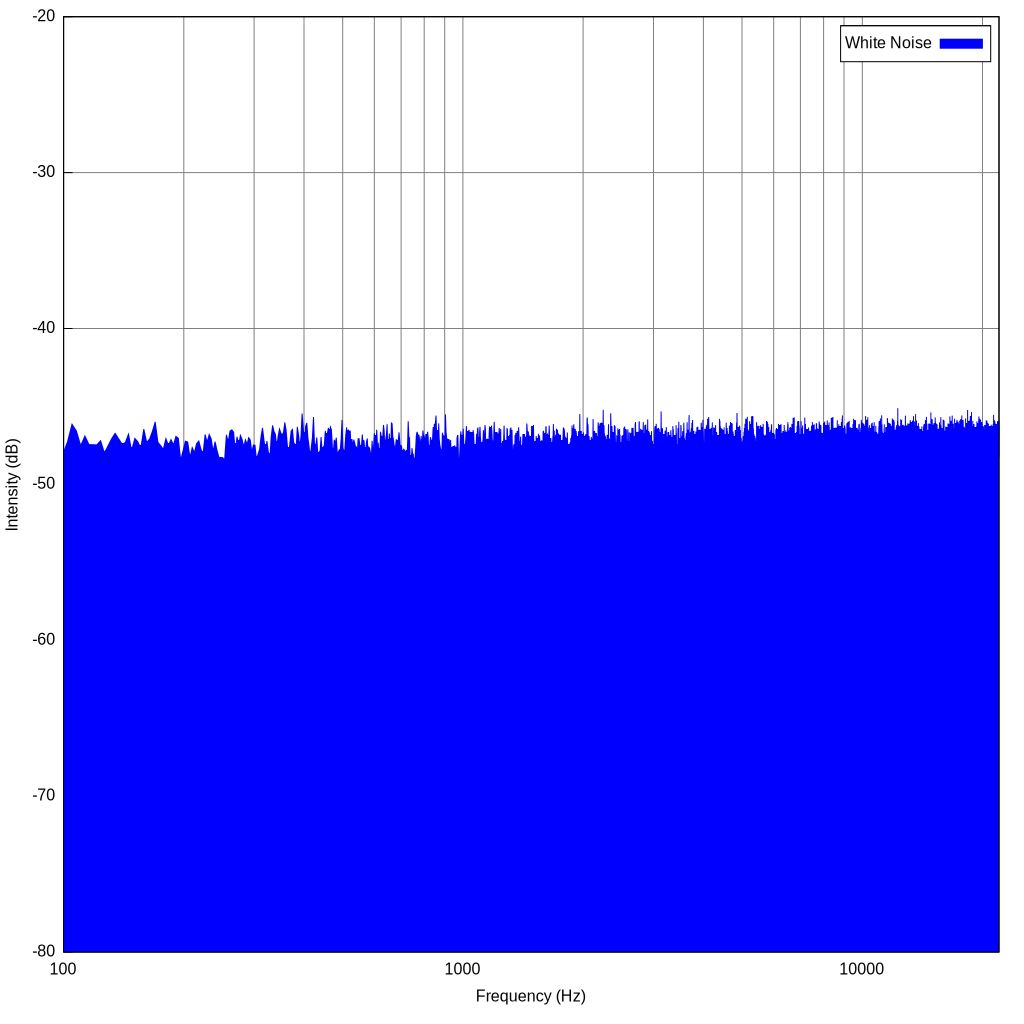
\includegraphics[valign=m,width=0.5\textwidth]{img/LSMessung/White_noise_spectrum.png}}
	\caption[Zeitfunktion und Spektrum von \enquote{weißem Rauschen}]{Zeitfunktion\footnotemark und Spektrum\footnotemark von \enquote{weißem Rauschen}}
	\label{fig:5.2.2.1}
\end{figure}
\footnotetext[2]{https://upload.wikimedia.org/wikipedia/commons/c/c1/White\_noise.svg}
\footnotetext[3]{https://upload.wikimedia.org/wikipedia/commons/3/3c/White\_noise\_spectrum.svg}
\begin{figure} [H]
	\centering
	%\includegraphics[width=1\textwidth]{img/LSMessung/modul.png}
	\caption{Messmodul}
	\label{fig:5.2.2.2}
\end{figure}

\newpage
\subsection{Verstärker}\label{subsec:5.2.3}
Prinzipiell kann für diesen Aufbau jeder Leistungsverstärker verwendet werden. In unserem Fall war ein \enquote{Brüel \& Kj\ae r Power Amplifier Type 2706} in Verwendung.\\
Da meist nur ein Lautsprecher gemessen wird, benötigt man auch nur ein Signal (Mono, kein Stereo) zum Messen. Der Verstärker verfügt über einen, in Stufen schaltbaren Abschwächer und einen stufenloses \enquote{Gain Control}.\\
Da auch andere Komponenten in dem Aufbau von der Firma  \enquote{Brüel \& Kj\ae r} sind, weist der Verstärker eine hohe Kompatibilität zum restlichen Equipment auf.
\begin{figure} [H]
	\centering
	%\includegraphics[width=1\textwidth]{img/LSMessung/verstärker.png}
	\caption{\enquote{Brüel \& Kj\ae r Power Amplifier Type 2706}}
	\label{fig:5.2.3.1}
\end{figure}

\subsection{Mikrofon}\label{subsec:5.2.4}
Um den Schalldruckpegel möglichst präzise messen zu können wird auch ein dementsprechend genaues Mikrofon benötigt. Das bei uns verwendete Mikrofon war das \enquote{Brüel \& Kj\ae r Type 2669}. \\
Ebenfalls wichtig ist die Ausrichtung des Mikrofons. Es sollte immer auf Höhe der Mitte des Lautsprechers angebracht werden. Die Entfernung muss bei verschiedenen Lautsprechern gleich bleiben, um vergleichbare Messungen zu ermöglichen. Bei einem Zwei-Weg-System (Hoch- und Tieftöner) haben wir das Mikrofon (vertikal gesehen) zwischen den Lautsprechern befestigt.
\begin{figure} [H]
	\centering
	\includegraphics[width=1\textwidth]{img/LSMessung/mikro.png}
	\caption{Messmikrofon \enquote{Brüel \& Kj\ae r Type 2669}}
	\label{fig:5.2.4.1}
\end{figure}
%\newpage
\section{Tieftöner-Messungen} \label{sec:5.3}
\subsection{Einleitung} \label{subsec:5.3.1}
Tieftöner sind, wie der Name bereits andeutet, für den unteren Frequenzbereich gedacht und konzipiert. In diesem Projekt werden Tieftöner-Lautsprecher an zwei verschiedenen Positionen verwendet:
\begin{itemize}
	\item Im Subwoofer und 
	\item in der Satellitenbox
\end{itemize}
Es ist so angedacht, dass der Subwoofer (Mono) nur die sehr niedrigen Frequenzen übernimmt. Er ist bis ca. 200 Hz aktiv.\\
In den Satellitenboxen ist jeweils ein kleinerer Tieftöner verbaut, um den Übergang zwischen sehr tiefen und hohen Frequenzen zu bilden. Diese zwei Lautsprecher (Stereo) arbeiten ebenfalls bei niedrigen als auch bei mittleren bis hohen Frequenzen. Die Grenze des Satelliten-Tieftöners liegt bei ca. 5 kHz.

\subsection{Ziele} \label{subsec:5.3.2}
Der Lautsprecher für die Subwoofer-Box muss größer und leistungsfähiger sein, um die richtig tiefen Frequenzen möglichst gut abzustrahlen. Da er nur bis ca. 200 Hz aktiv ist, sollte der Frequenzgang genau in diesem Bereich einen hohen Schalldruckpegel aufweisen. Der Rest des Frequenzganges ist nicht so wichtig, da der Lautsprecher auch nicht in einem höheren Bereich verwendet wird. \\
Bei den Satelliten-Lautsprechern ist der ganz tiefe Frequenzbereich nicht so ausschlaggebend. Wichtiger ist dafür eine niedrige Welligkeit bis 5 kHz, um den mittleren Frequenzbereich gut abstrahlen zu können.\\ \\
Der Messvorgang und -aufbau wurde bereits im Kapitel \ref{sec:5.2} erläutert. Nach diesem Prinzip wird bei fast allen Messungen vorgegangen.

\newpage
\subsection{Subwoofer} \label{subsec:5.3.3}
Bereits zu Beginn der Diplomarbeit wurde ein großer Tieftöner eingekauft. Dieser wurde in verschiedenen Volumina gemessen. Außerdem wurden Vergleichsmessungen mit einem zweiten Tieftöner durchgeführt.
\begin{figure} [H]
	\centering
	\includegraphics[width=0.5\textwidth]{img/LSMessung/TT/renkforce_B12123.png}
	\caption[\enquote{Renkforce B12123}]{\enquote{Renkforce B12123}\footnotemark}
	\label{fig:5.3.3.1}
\end{figure}
\footnotetext{https://www.conrad.at/de/auto-subwoofer-chassis-300-mm-500-w-renkforce-4-370335.html}
Dieser Lautsprecher wurde ausgewählt, weil er einen vergleichsweise hohen Schalldruckpegel bei tiefen Frequenzen aufweist. Kurze Spezifikationen des Subwoofers sind:
\begin{itemize}
	\item Maximale Belastbarkeit 500 W
	\item Durchmesser 30 cm
	\item Schalldruck 93 dB
	\item Impedanz 4 $\Omega$
\end{itemize}
Da man eine Box einfacher verkleinern kann als vergrößern, wurde eine Box mit einem Volumen von 149 l für die Messungen verwendet. Die Box wurde aus Holz gefertigt und mit Silikon abgeschlossen, um mögliche Luftlöcher zu schließen. Als Vergleichslautsprecher wurde ein \enquote{Visaton WPC30} gemessen.

\newpage
Diese Messungen wurden zu Beginn der Diplomarbeit durchgeführt und daher sind die Ergebnisse so aufgenommen, dass die Einstellungen der Software sichtbar sind.\\
Die zwei Subwoofer wurden einmal mit und einmal ohne Wolle in der Box gemessen. 
\begin{figure} [H]
	\centering
	\subfloat{\includegraphics[width=0.75\textwidth]{img/LSMessung/TT/RenkforceOhneWolleMitSilikon.png}}\quad
	\subfloat{\includegraphics[width=0.75\textwidth]{img/LSMessung/TT/VisatonMitSilikonOhneWolle.png}}
	\caption{Subwoofer-Messung ohne Wolle\\ \enquote{Renkforce} (oben) und \enquote{Visaton} (unten)}
	\label{fig:5.3.3.2}
\end{figure}
Bei diesem Vergleich ist sichtbar, dass der Frequenzgang des \enquote{Visaton}-Tieftöners allgemein \enquote{gerader} ist und weniger Welligkeit aufweist. Wenn man allerdings nur auf die tiefen Frequenzen achtet, die auch verwendet werden (<200 Hz), ist festzustellen, dass der Schalldruckpegel des \enquote{Renkforce} einen höheren Wert aufweist und daher zu bevorzugen ist.\\
Eine weitere Messung mit Wolle in der Box wurde deshalb durchgeführt, weil beide Frequenzgänge bei ca. 300 Hz einen Unregelmäßigkeit aufzeigen. Die Auswirkungen auf die Lautsprecher sind folgende:
\begin{figure} [H]
	\centering
	\subfloat{\includegraphics[width=0.75\textwidth]{img/LSMessung/TT/RenkforceMitWolleMitSilikon.png}}\quad
	\subfloat{\includegraphics[width=0.75\textwidth]{img/LSMessung/TT/VisatonMitSilikonMitWolle.png}}
	\caption{Subwoofer-Messung mit Wolle\\ \enquote{Renkforce} (oben) und \enquote{Visaton} (unten)}
	\label{fig:5.3.3.3}
\end{figure}
Beide Frequenzgänge wurden durch das Hinzufügen von Wolle etwas \enquote{glatter}, also haben weniger Welligkeit. Die Wolle kann z.B. stehende Wellen in der Box verhindern und verbessert so deshalb die Eigenschaften der gesamten Box.\\ \\
Der Lautsprecher \enquote{Renkforce} weist insgesamt bei tieferen Frequenzen einen höheren Schalldruckpegel auf und wurde auch deshalb von uns für dieses Projekt ausgewählt.

\subsection{Satelliten-Tieftöner} \label{5.3.4}













%\newpage
\section{Lautsprecher für Hochton-Bereich}
\input{tex/Weitere_Messungen.tex}


%% ANHANG ==============================================%%
\appendix

%% abkürzungsverzeichnis ===============================%%
%% start of file abkuerzungen.tex

% Abkuerzungsverzeichnis
\addchap{
	\iflanguage{english}{Acronyms}{Abkürzungsverzeichnis}}
\begin{acronym}[ACRONYM]
\acro{aux}[AUX-Input]{Auxilary Input - dt. Zusatz-Eingang}
%\acro{abb}[Abb.]{Abbildung}
\acro{bt}[BT]{Bluetooth}
\acro{cee}[CEE-Norm]{Commission on the Rules for the Approval of the Electrical Equipment - dt. internationale Kommission für die Regelung der Zulassung elektrischer Ausrüstungen}
%\acro{db}[dB]{Dezibel}
\acro{dek}[Dek.]{Dekade}
\acro{elko}[ELKO]{Elektrolyt-Kondensator}
\acro{emv}[EMV]{Elektro-Magnetische Verträglichkeit}
%\acro{f}[F]{Farat}
\acro{gpio}[GPIO]{General Purpose Input/Output - dt. Allzeckeingabe/-ausgabe}
\acro{hifi}[HiFi]{High Fidelity - dt. Hohe (Klang-)Treue}
\acro{ht}[HT]{Hochton-Lautsprecher}
\acro{HTBLuVA}[HTBLuVA]{Höhere Technische Bildungs, Lehr- und Versuchsanstalt}
%\acro{hz}[Hz]{Hertz}
\acro{ic}[IC]{Integrated Circuit - dt. Integrierter Schaltkreis}
%\acro{kap}[Kap.]{Kapitel}
\acro{led}[LED]{Light Emitting Diode - dt. Licht emittierende Diode}
\acro{Lipo}[LiPo]{Lithium Polimer}
\acro{opv}[OPV]{Operationsverstärker}
\acro{pcb}[PCB]{Printed Circuit Board - dt. Leiterplatte}
\acro{Rms}[RMS]{Rout-Mid-Square - dt. Effektivwert}
\acro{smd}[SMD]{Surface Mouted Device - dt. Auf der Oberfläche montierter Bauteil}
%%\acro{spi}[SPI]{Serial Peripheral Interface}
%%\acro{tikz}[TikZ]{\TikZ{} ist kein Zeichenprogramm}
\acro{tt}[TT]{Tiefton-Lautsprecher}
\acro{uart}[UART]{Universal Asyncron Reciev Transmitter - dt. Universelle Asynchrone Empfangs- und Übertragungsschnittstelle}
\acro{usb}[USB]{Universal Serial Bus - dt. Universaler Serieller Bus}
%\acro{v}[V]{Volt}
\acro{vbat}[VBAT]{Batterie Voltage - dt. Batteriespannung}
\acro{vcc}[Vcc]{Positive Versorgungsspannung}
\acro{via}[VIA]{Durchkontaktierungen einer Doppelseitigen-Leiterplate}
%\acro{zb}[zB.]{zum Beispiel}

% Hab mal das auskommentiert was meiner Meinung nach nicht unbedingt nötig ist ;)

\end{acronym}\newpage

%% end of file abkuerzungen.tex
%%======================================================%%

%% abbildungsverzeichnis ===============================%%
\setcounter{lofdepth}{2}
\dipalistoffigures
%%======================================================%%

%% tabellenverzeichnis =================================%%
\setcounter{lotdepth}{2}
\dipalistoftables
%%======================================================%%

%% danksagungen=========================================%%
\newpage
\begin{acknowledgements}
    Wir bedanken uns bei
    \subparagraph{Prof. Dipl.-Ing. Dr. Herbert Wagner} für die tatkräftige Unterstützung und das ermöglichen eines einwandfreien Arbeitens an unserer Diplomarbeit und dem Projekt.
    %\subparagraph{FL Ing. DEFG} für ...
\end{acknowledgements}

%%======================================================%%

%% literaturverzeichnis ================================%%
\newpage
\begin{literature}
% The TeXbook by D. E. Knuth
%\bibitem[1]{TeXbooooook}{\textbf{Donald~E.~Knuth:} \emph{The \TeX{}book}. 1986, {\scshape Addison--Wesley} Verlag,\\ ISBN-13: 978-0-201-13447-6}
\bibitem[1]{TDA2030Amp}{\textbf{Herbert Sax:} SGS-Ates TDA2030 , {\scshape SGS-Ates} Verlag,\\ ISBN-13: -}

\end{literature}
 
%%======================================================%%

%% betreuungsprotokolle ================================%%
\includepdf[pages=-]{form/betreuungsprotokoll_1.pdf}
\includepdf[pages=-]{form/betreuungsprotokoll_2.pdf}
%% =====================================================%%

\end{document}
